\documentclass[problem]{mcs}

\begin{pcomments}
  \pcomment{PS_choose_isomorphic_graphs}
  \pcomment{from: S09.ps5; S06.ps4; F07.ps5; F06}
  \pcomment{in S06 essentially taken from the Course Notes for the
            University of Waterloo class C&O 230; add citation}
\end{pcomments}

\pkeywords{
  graphs
  isomorphisms
  bijections
}

%%%%%%%%%%%%%%%%%%%%%%%%%%%%%%%%%%%%%%%%%%%%%%%%%%%%%%%%%%%%%%%%%%%%%
% Problem starts here
%%%%%%%%%%%%%%%%%%%%%%%%%%%%%%%%%%%%%%%%%%%%%%%%%%%%%%%%%%%%%%%%%%%%%

\begin{problem}
Determine which among the four graphs pictured in the Figures 
%~\ref{fig:isog}
are isomorphic.  If two of these graphs are isomorphic, describe an
isomorphism between them.  If they are not, give a property that is
preserved under isomorphism such that one graph has the property, but the
other does not.  For at least one of the properties you choose,
\emph{prove} that it is indeed preserved under isomorphism (you only need
prove one of them).

\begin{figure}[h] %[htbp]
\begin{center}
\mbox{  \subfloat[$G_1$]{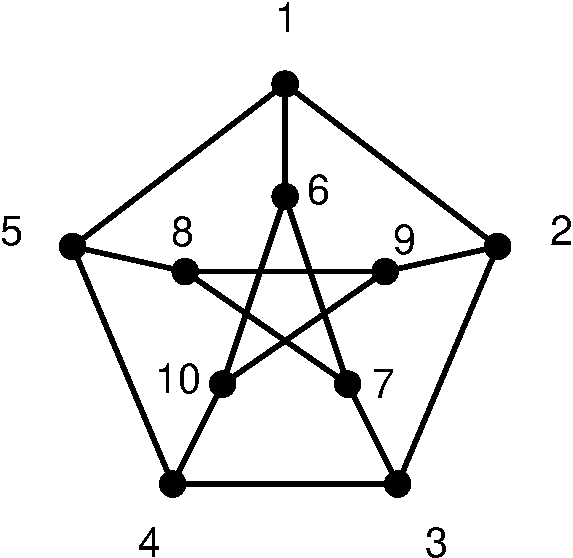
\includegraphics[width=1.5in,clip]{figures/G1}}
        \hspace{17mm}
        \subfloat[$G_2$]{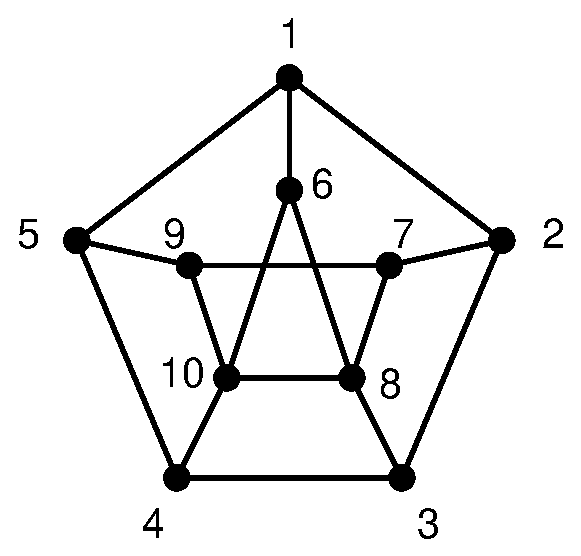
\includegraphics[width=1.5in,clip]{figures/G4}} }
\mbox{  \subfloat[$G_3$]{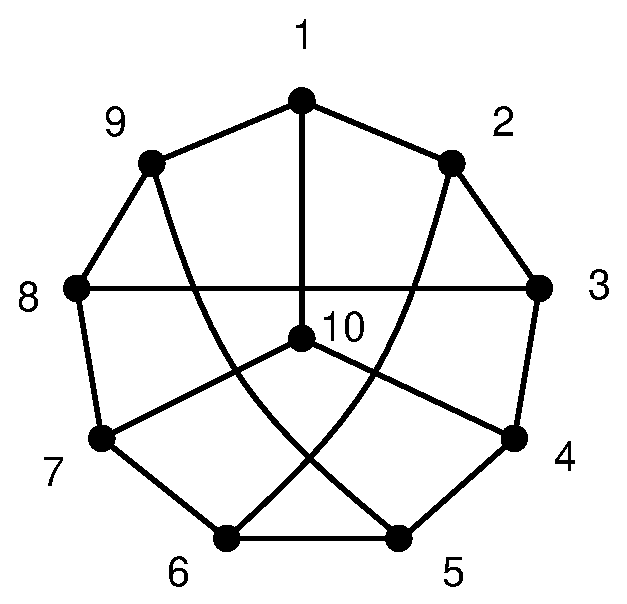
\includegraphics[width=1.5in,clip]{figures/G2}}
        \hspace{17mm}
        \subfloat[$G_4$]{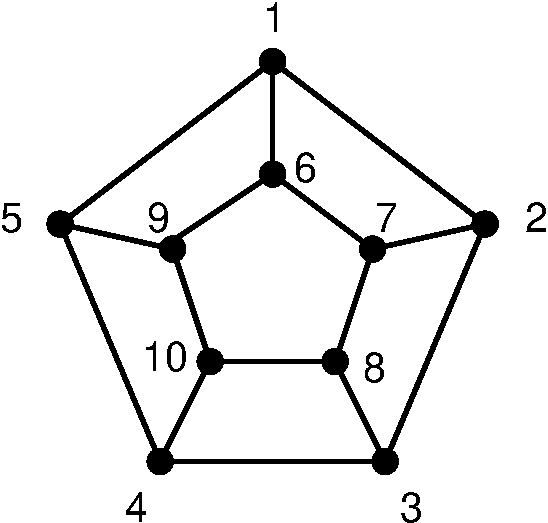
\includegraphics[width=1.5in,clip]{figures/G3}}
        }
\end{center}
\caption{Which graphs are isomorphic?}
\label{fig:isog}
\end{figure}

\iffalse


\begin{figure}[h] %[htbp]
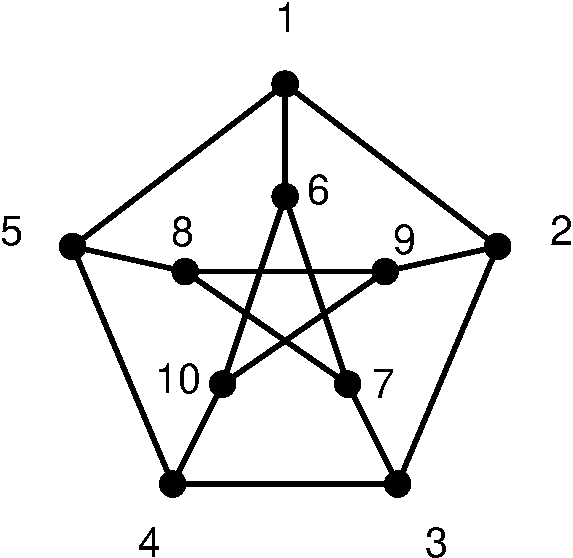
\includegraphics[width=1.5in,clip]{figures/G1}
\caption{$G_1$}
\label{fig:G1}
\end{figure}


\begin{figure}[h] %[htbp]
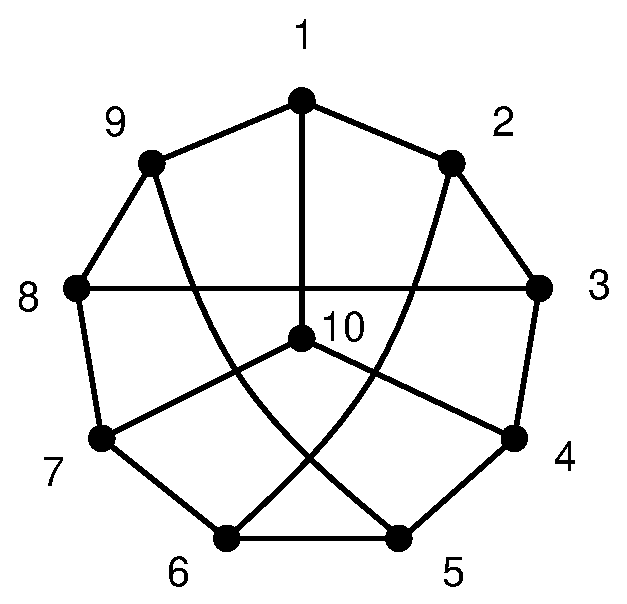
\includegraphics[width=1.5in,clip]{figures/G2}
\caption{$G_2$}
\label{fig:G2}
\end{figure}


\begin{figure}[h] %[htbp]
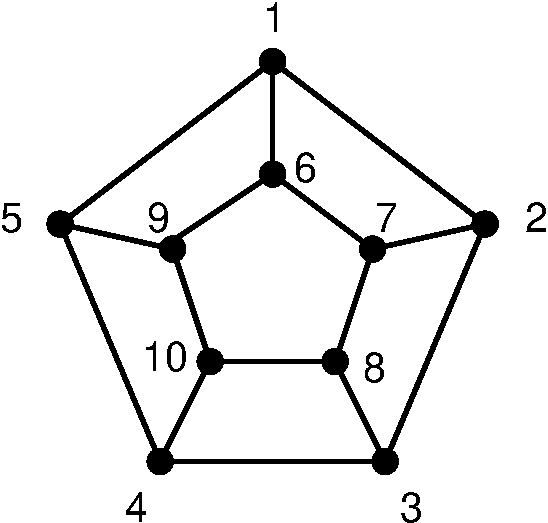
\includegraphics[width=1.5in,clip]{figures/G3}
\caption{$G_3$}
\label{fig:G3}
\end{figure}

\begin{figure}[h] %[htbp]
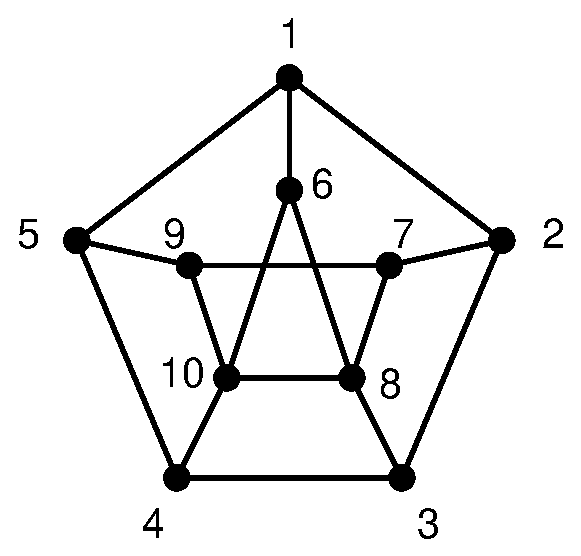
\includegraphics[width=1.5in,clip]{figures/G4}
\caption{$G_4$}
\label{fig:G4}
\end{figure}
\fi

\begin{solution}
$G_1$ and $G_3$ are isomorphic.  In particular, the function
$f:V_1 \to V_3$ is an isomomorphism, where
\begin{align*}
&f(1)=1 \quad&& f(2)=2 \quad&& f(3)=3 \quad&& f(4)=8 \quad&& f(5)=9 \\
&f(6)=10 \quad&& f(7)=4 \quad&& f(8)=5 \quad&& f(9)=6 \quad&& f(10)=7
\end{align*}

$G_1$ and $G_4$ are not isomorphic to $G_2$: $G_2$ has a vertex of degree
four and neither $G_1$ nor $G_4$ has one.

$G_1$ and $G_4$ are not isomorphic: $G_4$ has a simple cycle of length
four and $G_1$ does not.


\textbf{There are many examples of properties preserved under graph isomorphism. We accepted any that were used.}

For example, we will prove that the degree of each vertex is preserved under isomorphism.

Let $G$ and $H$ be isomorphic graphs. Since they are isomorphic, there is an edge-preserving bijection between the vertices of $G$ and $H$:

$f:u \in V(H) \iff f(u) \in V(G)$
 
We let the set of vertices adjacent to $u$ be $n(u)$. Because $f$ is an edge-preserving bijection, there is an edge from $f(u)$ to a vertex $f(k)$ iff $k \in n(u)$. 
Thus $|n(f(u))| = |n(u)|$ and the degree of each vertex is preserved under isomorphism.

\end{solution}

\end{problem}

%%%%%%%%%%%%%%%%%%%%%%%%%%%%%%%%%%%%%%%%%%%%%%%%%%%%%%%%%%%%%%%%%%%%%
% Problem ends here
%%%%%%%%%%%%%%%%%%%%%%%%%%%%%%%%%%%%%%%%%%%%%%%%%%%%%%%%%%%%%%%%%%%%%

\endinput
